\part{Energia Fotovoltaica}
\chapter[Energia Fotovoltaica]{Energia Fotovoltaica}

\section{Introdução}

O efeito fotovoltaico foi observado em 1839 pelo físico francês Alexandre Edmond Becquerel. Quando incidindo, sobre uma superfície semicondutora, uma luz ele observou a diferença de potencial entre suas extremidades.

As primeiras células fotovoltaicas surgiram em 1956, com o grande desenvolvimento da microeletrônica, mas o alto custo já tornava a popularização de sua utilização inviável, eram empregadas comumente em sistemas espaciais para o fornecimento de energia elétrica. Essa utilização se dava pelo balanço de custo das placas em relação ao sistema espacial como um todo que tornava as placas não tão inviáveis, além de seu baixo peso e bom desempenho em ambiente espacial.

Com a crise do petróleo em 1973 foi impulsionada fortemente a pesquisa e desenvolvimento da tecnologia fotovoltaica para diversas aplicações, esse tipo de produção de energia elétrica passou a atrair uma maior atenção dos governos. Entretanto, um fator ainda preocupante era a baixa eficiência das células fotovoltaicas em relação ao seu custo de produção, nisso o mercado tem ainda um desenvolvimento muito lento. Em 1978 a produção das células chegava a 1 Mwp/ano, quinze anos depois já alcançava 60 Mwp/ano, já em em 1998 a produção prevista era em torno de 100 Mwp/ano \cite{do2004principio}.

Atualmente a viabilidade de utilização das placas fotovoltaicas não está em necessariamente criar uma grande usina para abastecimento geral, mas em pequenas instalações em locais urbanos (casas, prédios, parques) que são capazes de suprir a demanda pontual e até mesmo fornecer energia elétrica gerada excedente, ou locais rurais que ainda dependem de fontes como carvão e biomassa para diminuir a dependência de fontes muito poluentes. 

\subsection{Efeito fotovoltaico}

Células fotovoltaicas são fabricadas com material semicondutor, um material que possui características intermediárias entre condutor e isolante. Para essas células é utilizado, basicamente, o silício como material semicondutor. 
	
O silício é um material bastante abundante na superfície terrestre, normalmente encontrado na areia e, para utilização na fabricação das células fotovoltaicas é extraído, muitas vezes, de forma mais pura possível através de métodos adequados. O cristal de silício puro é um mal condutor pela ausência de elétrons livres em sua composição, para que estre passe a conduzir acrescenta-se quantidades de outros elementos ao cristal, este processo é denominado dopagem.

A dopagem do silício com fósforo gera um material com elétrons livre, portadores de cargas negativas excedentes, denominado silício tipo N. Já a dopagem do silício com o elemento boro gera um material com características inversas, este é portador de cargas positivas excedentes, silício tipo P.

As células fotovoltaicas são compostas por uma placa fina de silício tipo N acoplada à uma placa com maior espessura de silício tipo P, unidas formam uma região P-N, onde há um campo elétrico devido a diferença de potencial entre as placas, naturalmente os elétrons fluirão no sentido N para P até que o equilíbrio seja atingido. Quando a célula é exposta à luz, os fótons excitam os elétrons da região N, fazendo com que continuem a fluir para a região P, gerando, assim, uma corrente contínua. A figura \ref{fig:fotovoltaica} apresenta informações mais detalhadas a respeito das células fotovoltaicas, os tipos de painéis, a eficiência e a duração. 

\subsection{Vantagens e Desvantagens}

São muitas as vantagens da utilização de um sistema fotovoltaico, pois ele é uma geração não prejudicial ao meio ambiente e durante sua produção de energia elétrica não há nenhum tipo de poluição. As placas possuem vida útil muitas vezes superior a 25 anos com uma manutenção adequada e a utilização de uma fonte inesgotável, o Sol.

As principais vantagens são:

\begin{itemize}
	\item Não consome combustível;
	\item Não produz poluição;
	\item É uma fonte silenciosa;
	\item A vida útil é superior a 25 anos;
	\item Resistente a condições climáticas (umidade, altas temperaturas, vento, chuvas);
	\item Manutenção simples (a limpeza dos painéis é a única manutenção realmente rotineira);
	\item Capacidade de geração até em dias não ensolarados (mesmo com eficiência baixa);
	\item Possibilidade de ajustes na potência instalada através da incorporação ou retirada de módulos;
\end{itemize}

A geração de energia elétrica através do efeito fotoelétrico, em comparação a outras fontes, apresenta uma série de desvantagens. A eficiência é baixa quando analisada a possibilidade de aproveitamento, pois há muitos fatores que reduzem a eficiência, como exemplo: reflexão e sombreamento na placa, excedência e insuficiência de energia do fóton nas radiações de onda curta e longa, respectivamente, entre outros. Ainda há a questão ambiental envolvendo não a produção da energia elétrica, mas a fabricação das células, o processo de purificação do silício é tão prejudicial ao meio ambiente quanto qualquer outro processo industrial.

As principais desvantagens são:

\begin{itemize}
	\item As células fotovoltaicas necessitam de tecnologia sofisticada para sua produção;
	\item O custo para implementação de um sistema fotovoltaico é elevado;
	\item A eficiência das células não alcança índices muito altos;
	\item O rendimento depende de fatores sempre presentes, como nuvens e radiação solar;
	\item Não há produção de energia elétrica durante a noite para abastecimento.

\end{itemize}

\cite{braga2008energia}.

\section{Funcionamento de um Sistema Fotovoltaico}

Um sistema fotovoltaico é um conjunto de componentes que possibilitam a transformação de energia luminosa (cuja fonte é o sol) em energia elétrica \cite{ecycleconheca}. O sistema é dividido em três blocos principais:

\begin{itemize}
	\item Bloco Gerador: É o responsável pela transformação de energia
	\item Bloco de condicionamento de potência: É responsável por adaptar a energia gerada para a utilização final.
	\item Bloco Armazenador: Responsável pelo o armazenamento da energia elétrica.
\end{itemize}

Além disso, os sistemas fotovoltaicos podem se apresentar em diferentes configurações, sendo elas de acordo com \cite{creseb2006energia}:

\begin{itemize}
	\item Sistemas Isolados: Desconectado da rede de energia
	\item Sistemas Híbridos: Diferentes tipos de geração de energia ligados a uma mesma rede.
	\item Sistemas conectados à rede: A energia gerada pelo sistema é distribuída diretamente na rede convencional.
\end{itemize}

A junção dos três blocos citados acima, colocados em uma configuração adequada ao local de instalação do complexo compõem o Sistema Fotovoltaico. 

\subsection{Bloco Gerador}

O bloco gerador é composto por módulos fotovoltaicos, estruturas de suporte e cabeamento.

O funcionamento da energia solar fotovoltaica ocorre quando os painéis fotovoltaicos são expostos a partículas de luz solar, essas partículas são chamadas de fótons. Eles fazem a trajetória entre o Sol e a Terra por cerca de 9 minutos.  Ao atingir as células fotovoltaicas, os elétrons que são transportados pelo semicondutor e circulam em torno dos átomos se desprendem deixando espaços vazios. Durante a exposição, através de corrente elétrica, esses se deslocam em direção constante a célula de silício, que está com ausência de elétrons. Este fluxo intenso de elétrons,  gera a energia solar fotovoltaica. Os elétrons continuam a se livrar dos átomos, enquanto há incidência de luz solar.

Um módulo fotovoltaico é um conjunto de placas fotovoltaicas, ligadas em série ou em paralelo, que fornecem certa corrente e tensão final. O módulo fotovoltaico também é chamado de painel fotovoltaico.

A ligação de módulo pode ser feita de duas formas, em série ou em paralelo. O arranjo em série consiste em agrupar o maior número de células possível até alcançar a tensão de 12V, a tensão final será a soma da tensão de cada uma das células. Esse arranjo é o mais comum em sistemas fotovoltaicos.

\begin{figure}[!h]
\centering
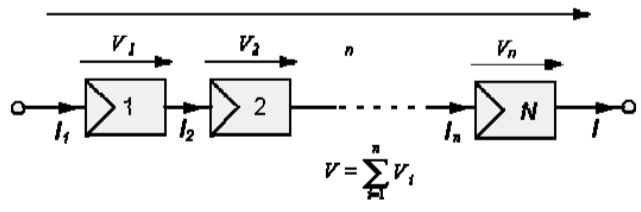
\includegraphics[width=0.5\textwidth]{figuras/associacao.png}
\caption{Esquema de associação de células fotovoltaicas em série}
\label{fig:associacao}
\end{figure}

Já o arranjo em paralelo fornece a corrente contínua final como a soma das correntes de cada placa e a tensão como a tensão de uma única placa. Esse arranjo é pouco utilizado já que a tensão fica em torno de 0,7V e a corrente máxima em 3A \cite{da2008projeto}.

\begin{figure}[!h]
\centering
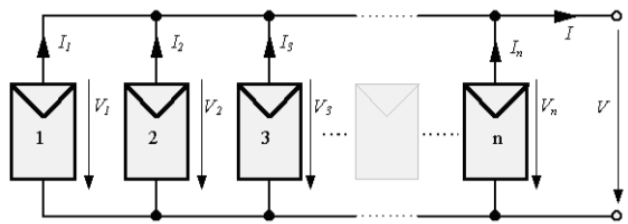
\includegraphics[width=0.5\textwidth]{figuras/associacaoserie.png}
\caption{Esquema de associação de células fotovoltaicas em paralelo}
\label{fig:associacaoparalelo}
\end{figure}

As estruturas de suporte são estruturas que suportam os módulos solares, eles podem ser fixos e sem angulação, voltados constantemente para cima. Podem ser móveis com angulação que é mudada manualmente de acordo com as condições anuais. E podem ser dispositivos tracker, estruturas automatizadas que mudam de angulação segundo a posição do sol durante os dias \cite{ecycleconheca}. 

Já o cabeamento corresponde a todo o conjunto de cabos que são necessários para a interligação dos componentes do sistema fotovoltaico. Em geral, são utilizados cabos do tipo módulo ou fileira, que protegem o sistema contra curto-circuitos e falhas \cite{ecycleconheca}.

\subsection{Bloco de condicionamento de potência}

O bloco de condicionamento de potência é composto por um inversor e um controlador de carga.

Os inversores são conversores de corrente contínua em corrente alternada (CC/CA). A maioria dos aparelhos utiliza corrente alternada enquanto o módulo fotovoltaico produz corrente contínua, por isso a necessidade de se instalar um no sistema fotovoltaico. O inversor funciona “quebrando” a corrente contínua em pulsos, isso permite que ela se torne alternada. Eles podem ser divididos em seis categorias de acordo com \cite{neosolaronda}:

\begin{enumerate}
    \item Onda Quadrada: são os mais baratos e econômicos, geram pulsos alternados, mas são pouco recomendados. Usados apenas para pequenas aplicações.
	\item Inversores de onda senoidal modificada: Muito utilizado, recomendado para pequenas instalações. Possui uma onda entre a senoidal pura e a quadrada.
	\item Inversores de onda senoidal pura: Tem sido cada vez mais utilizado por ter preço parecido com os de onda senoidal modificada, pode ser ligado a qualquer aparelho. E possui um tipo de onda senoidal quase pura. 
	\item Inversores para conexão à rede (Grid-Tie): Necessário se o sistema for interligado à rede. Além de produzir uma onda senoidal quase pura, alinha a frequência com a frequência da rede elétrica.
	\item Microinversores para conexão à rede (Grid-Tie): Cada vez mais utilizado, por ser de mais fácil instalação, ligado a cada placa individualmente, além de ter uma maior durabilidade.
	\item Inversor/Carregador: Além de agir como um inversor é capaz de agir carregando uma bateria ligada à uma fonte de CC, isso permite reduzir a quantidade de baterias necessárias no bloco de armazenamento.
\end{enumerate}

Os controladores de carga são ligados ao bloco de armazenamento e controla a carga e a descarga das baterias, aumentando assim a vida útil das mesmas. Se a bateria descarrega rapidamente em longos períodos sem insolação o controlador impede que a bateria se descarregue completamente, já em períodos de grande insolação, o controlador impede a carga excessiva.

Os controladores de carga podem ser divididos em três grandes grupos principais \cite{da2008projeto}: 

\begin{enumerate}
    \item Reguladores Série: Incorporam um interruptor entre o gerador e o acumulador, para interromper o fluxo e energia para a carga.
	\item Reguladores Shunt (derivação): O interruptor curta-circuita o gerador solar em fim de carga.
	\item Reguladores de ponto de potência máxima (MPPT): Utilizam um circuito eletrônico que sempre tende a captar a potência máxima. 
\end{enumerate}

\subsection{Bloco Armazenador}

O bloco armazenador é composto por baterias que armazenam a energia produzida para ser utilizada em períodos de mau tempo ou durante a noite. Existem vários tipo de bateria, cada uma adequada a situações específicas. Segundo \cite{ecycleconheca}, dentre elas temos:

\begin{enumerate}
    \item Baterias de Chumbo-Ácido: São as mais utilizadas para sistemas fotovoltaicos devido à grande variedade de tamanhos, baixo custo e bom desempenho. As mais comuns são: Chumbo-Antimônio, Chumbo-Selênio e Chumbo-Cálcio.
	\item Baterias de Chumbo-Ácido com eletrolito captativo: Também chamadas de baterias de chumbo-ácido com válvula reguladora. São de fácil transporte e podem ser instaladas em locais isolados. O ponto fraco é a excessiva sobrecarga e a perda do eletrólito , que é acelerado para clima quentes.
	\item Baterias de Níquel-Cádmio:  São utilizadas em sistemas fotovoltaicos isolados devido ao seu longo tempo de vida, pequena manuntenção, sobrevivencia a excessivas sobrecargas, excelente capacidade de retenção a baixas temperaturas e não necessidade de ter uma tensão de regulação de carga. As desvantagens são o grande custo e a necessidade de aplicação especifica. 
\end{enumerate}

\subsection{Configurações de sistemas fotovoltaicos}

Já em relação à configuração de um sistema fotovoltaico temos três tipos:

\begin{enumerate}
    \item Sistema Isolado: Também chamado de off-grid, se caracteriza por não se conectar à rede elétrica. É construído com lugar e propósito específico abastecendo diretamente o aparelho a ser utilizado. Um exemplo de sistema isolado é a iluminação pública \cite{neosolarisolado}. 
	\item Sistema Híbrido: Consiste de duas ou mais fontes de energia renováveis utilizadas em conjunto para proporcionar uma maior eficiência no sistema, bem como um maior equilíbrio no fornecimento de energia.  Um exemplo é a utilização de energia fotovoltaica e eólica em um mesmo sistema \cite{ecoplanetenergy}. 
	\item Sistema conectado à rede: Também chamado de On-Grid, o sistema é interligado à rede comum de distribuição de energia, assim não é necessário um sistema de armazenamento. Durante o período de pouca insolação ou durante à noite, a energia utilizada para abastecer o local passa a ser da rede comum. Já se a produção da energia solar excede à consumida, essa energia passa para a rede compartilhada e produz uma diminuição no consumo de energia \cite{solarbrasil}. 
\end{enumerate}

\begin{figure}[!h]
\centering
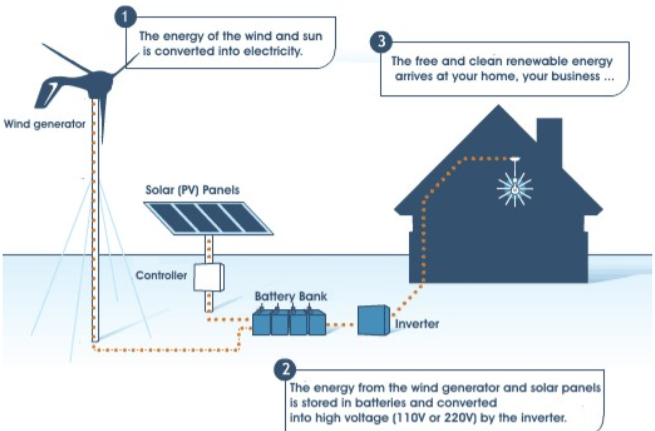
\includegraphics[width=0.5\textwidth]{figuras/esquema.png}
\caption{Esquema de energia híbrida (Fotovoltaiva e Eólica)}
\label{fig:esquema}
\end{figure}

\begin{figure}[!h]
\centering
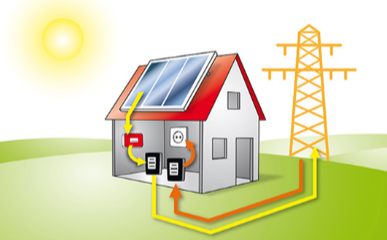
\includegraphics[width=0.5\textwidth]{figuras/ongrid.png}
\caption{Representação esquemática do sistema On-Grid. Cores Fantasia.}
\label{fig:ongrid}
\end{figure}

\section{Incidência solar na FGA}

Além das condições atmosféricas, a disponibilidade de radiação solar, ou energia total incidente sobre a superfície terrestre, depende da latitude local e da posição no tempo (hora do dia e do ano). 

Segundo dados do \cite{colle1998atlas} mostrado na figura \ref{fig:atlas}, Brasília é uma região que recebe aproximadamente de 5700 a 5900 Wh por $m^{2}$ todos os dias, o que representa uma alta quantidade de energia solar recebida também na região onde se concentra a Faculdade UnB Gama. 

\begin{figure}[!h]
\centering
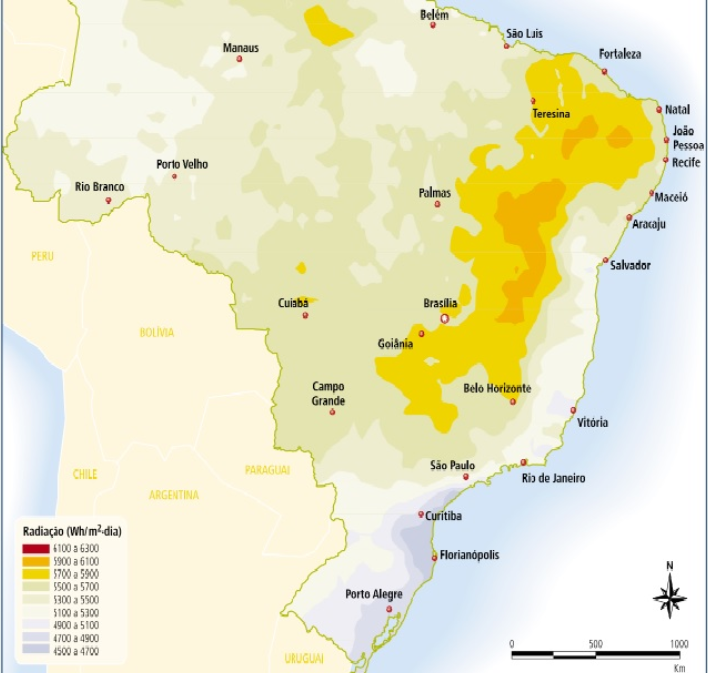
\includegraphics[width=0.75\textwidth]{figuras/atlas.png}
\caption{Fonte: \cite{colle1998atlas}}
\label{fig:atlas}
\end{figure}

Outro dado importante diagnosticado pelo ATLAS Solarimétrico do Brasil, Brasília recebe em média anualmente 6 horas de insolação por dia. 

Para tornar máximo o aproveitamento da radiação solar, o sistema solar fotovoltaico pode ser instalado com uma angulatura específica para a localidade, que depende da latitude do local e do período do ano que se deseja obter mais energia. Como podemos ver na figura \ref{fig:planoinclinado}, o gráfico de irradiação solar da UNB campus Gama:

\begin{figure}[!h]
\centering
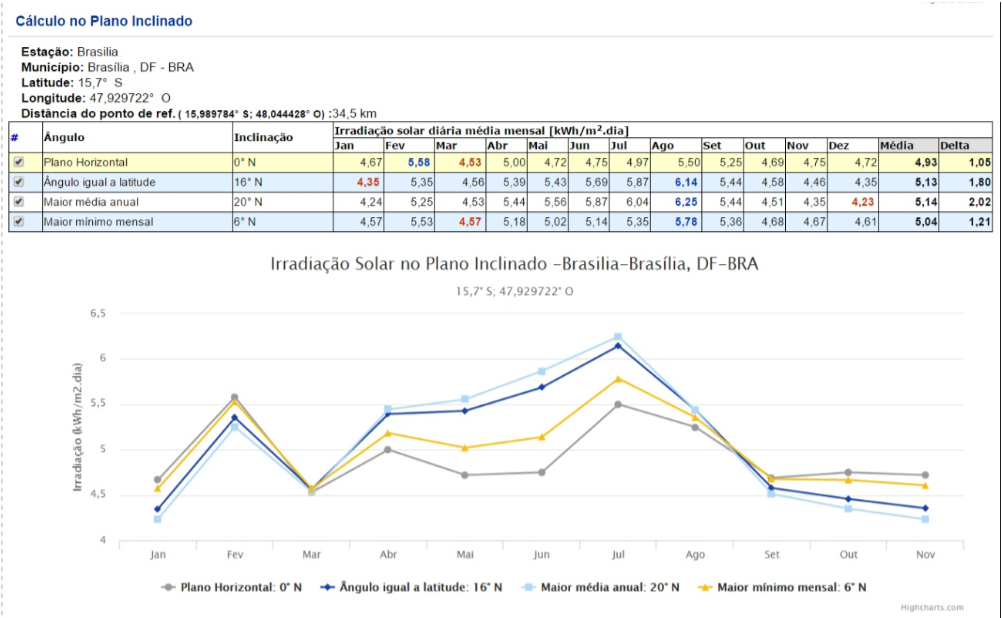
\includegraphics[width=0.75\textwidth]{figuras/planoinclinado.png}
\caption{Gráfico de irradiação solar da UnB campus Gama}
\label{fig:planoinclinado}
\end{figure}

Neste gráfico estão contido valores de radiação solar que será absorvido (KWh/$m^{2}$ dia) ao longo dos meses a partir do SunData do CRESESB, no qual já pode ser verificado a melhor angulação a serem colocadas as placas conforme a coordenada do campus. Verifica-se a partir deste gráfico que a angulação de 20º é a melhor, pois possui um delta total  (diferença da maior irradiação para a menor irradiação) e média anual de irradiação maior que as demais angulações. A aplicação que será feita está de forma detalhada no desenho.

\section{Manutenção das placas}

A manutenção das placas se dará de forma simples e manual, visto que a poeira do local de instalação das placas é considerada bastante acentuada e que, se essa poeira revestir os painéis fotovoltaicos, o rendimento na geração de energia será muito baixo ou quase nenhum. Essa limpeza acontecerá de acordo com a quantidade de poeira existente nas placas e a diminuição de rendimento. Ter-se-á todo controle de rendimento e quando este diminuir a limpeza será feita. Inicialmente, os funcionários da limpeza poderão lavar as placas com água e sabão neutro. Posteriormente, e se houver iniciativa de alunos e professores do curso de energia, alunos participantes de projeto poderão fazer a limpeza das placas, visto que, de acordo com alguns estudantes, não se tem muita prática nas aulas de fontes de energia, além da facilidade de se fazer tal limpeza. Essa iniciativa poderia ajudar alunos que se interessam na área de energia fotovoltaica a medir eficiência na prática e ajudar na manutenção dessas placas.

\begin{figure}[!h]
\centering
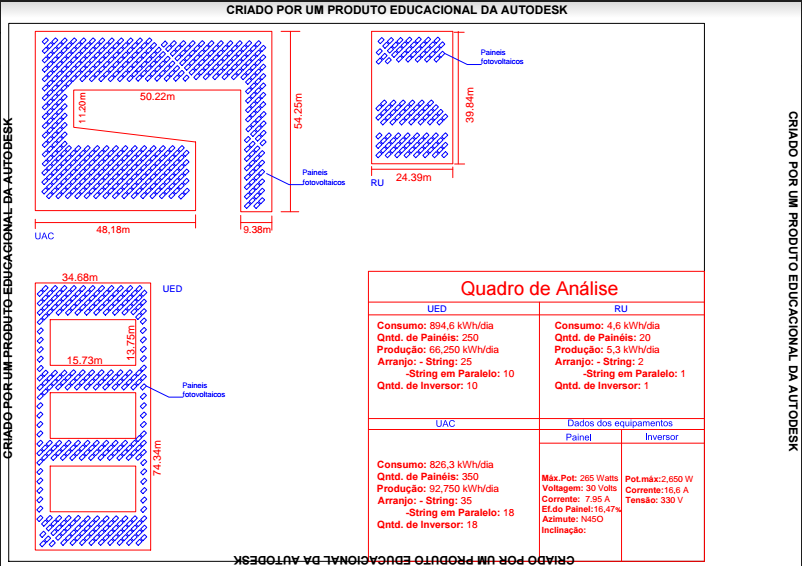
\includegraphics[width=0.75\textwidth]{figuras/fotovoltaica.png}
\caption{Desenho esquemático da manutenção de placas fotovoltaicas}
\label{fig:fotovoltaica}
\end{figure}

\section{Tipos de painéis solares fotovoltaicos}

O painel solar é o componente principal de um sistema de geração de energia solar, formado por um conjunto de células fotovoltaicas que geram energia através da luz solar. Quando  as células são atingidas pelos raios solares, os elétrons se movimentam, gerando a corrente elétrica.

A escolha do tipo e da quantidade de painéis adequados depende da demanda de uso e do local de instalação. Dentre vários tipos existentes, foi escolhido três distintos, porém básicos, sendo eles: Monocristalino, Policristalino e Silício amorfo (a-Si).

\subsection{Painel Solar Monocristalino}

É mais eficiente e produzido de células monocristalinas de silício. O silício deve ter um elevado grau de pureza que torna o processo complexo para a produção de cristais únicos para cada célula. Os painéis possuem uma eficiência média de 14\% - 21\%, estão disponíveis nas cores: azul escuro ou quase preto (com anti reflexo), cinza ou azul acinzentada( sem anti reflexo) e possuem formato arredondado. São mais caros que o policristalino e possuem vida útil maior que 30 anos, com garantia de fábrica de 25 anos. As vantagens do painel monocristalino é  que possui a eficiência mais alta dentre as tecnologias comercialmente viáveis atualmente e ocupam menor espaço. As desvantagens se dão por conta dos custos serem maiores e por desperdiçar uma certa quantia de silício na hora da produção \cite{neosolar}.

\begin{figure}[!h]
\centering
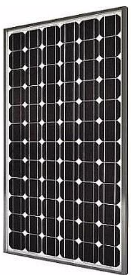
\includegraphics[width=0.3\textwidth]{figuras/placa.png}
\caption{Painel Solar Monocristalino}
\label{fig:placa}
\end{figure}

\subsection{Painel Solar Policristalino}

São menos eficiente que os monocristalinos e são formadas por diversas células, tornando-os diferente dos monocristalinos, o que dá uma aparência de vidro quebrado á célula. Tem eficiência média de 13\% - 16,5\%, está disponível na cor azul e é encontrado na forma quadrada. Possui vida útil de 30 anos e com garantia do fabricante de 25 anos. As suas vantagens se dão pelo fato da quantidade de resíduos de silício gerado ser menor que os monocristalinos e por ter um custo menor. Já as desvantagens: Serem menos eficientes que os monocristalinos, e precisarem de uma área maior para gerar a mesma quantidade de energia que os painéis monocristalinos \cite{neosolar}.

\begin{figure}[!h]
\centering
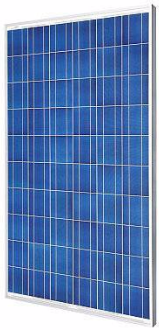
\includegraphics[width=0.3\textwidth]{figuras/painel.png}
\caption{Painel Solar Policristalino}
\label{fig:painel}
\end{figure}

\subsection{Painel de silício amorfo (a-Si)}

A produção de energia nessa tecnologia é baixa, as células solares de silício amorfo eram usadas para aplicações de pequenas escalas, tais como: calculadoras de bolso. Portanto, hoje já está sendo disponível para ser utilizada em larga escala.  Utiliza de uma técnica chamada de empilhamento, na qual várias camadas de células solares de silício amorfo são combinadas, resultando numa taxa de 6\% - 9\% de eficiência. A vantagem é que são necessário apenas 1\% do silício utilizado em células solares de silício cristalino. Já a desvantagem é que a técnica do empilhamento tem custos elevados \cite{neosolar}.

\begin{figure}[!h]
\centering
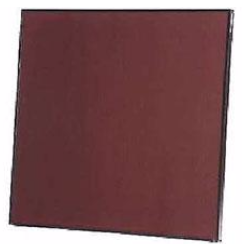
\includegraphics[width=0.3\textwidth]{figuras/marrom.png}
\caption{Painel Solar silício amorfo}
\label{fig:marrom}
\end{figure}

\section{Especificações e preços}
Após as várias pesquisas que foram realizados e levantamento de orçamentos a equipe foi capaz de determinar quais são as melhores opções para esse tipo de projeto, a ser realizado. Os materiais e quantidades foram detalhados e orçados em sites de compras On-line, uma vez que analisados os preços das lojas locais de encontrou uma disparidade de preços muito grande e as mesmas não possuem grandes quantidades desses tipos de produtos em estoque.

\par Para a escolha das marcas, foi feito um levantamentos sobre o que é necessário, de acordo com as especificações técnicas, e separado em uma tabela (Tabela \ref{tab:qtd}) com o intuito de organização.

\begin{table}[]
\centering
\caption{Quantidades necessárias e menores valores encontrados}
\label{tab:qtd}
\begin{tabular}{|l|c|c|c|}
\hline
\multicolumn{1}{|c|}{\textbf{Componente}} & \textbf{Quantidade} & \textbf{Valor unitário} & \textbf{Valor total} \\ \hline
Painel Fotovoltaico                       & 620                 & R\$ 849,00              & R\$ 526.380,00       \\ \hline
Inversor                                  & 29                  & R\$ 14.190,00           & R\$ 411.510,00       \\ \hline
Fiação para sistemas fotovoltaicos        & 600                 & R\$ 4,69                & R\$ 2.814,00         \\ \hline
Suporte de angulação                      & 620                 & R\$ 110,00              & R\$ 68.200,00        \\ \hline
Presilhas para módulos (placas)           & 2480                & R\$ 2,80                & R\$ 6.944,00         \\ \hline
Quadros e disjuntores                     & 62                  & R\$ 1.290,00            & R\$ 72.980,00        \\ \hline
\end{tabular}
\end{table}

\subsection{Módulos fotovoltaicos}
Após a análise mais detalhada dos tipos de placas fotovoltaicas existentes, chegou-se a um consenso de que as placas Policristalinas, placas que contém um ``compensado'' de silício, seria a melhor opção para esse investimento. A marca Canadian se mostra uma das empresas mais promissoras no mercado e teve o melhor custo benefício.

\begin{figure}[h]
\centering
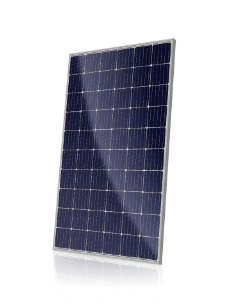
\includegraphics[width=0.5\textwidth]{figuras/painel1.PNG}
\caption{Painel Fotovoltaico Canadian 265W}
\end{figure}

ESPECIFICAÇÕES TÉCNICAS DO PAINEL DE 265 Wp DE ENERGIA SOLAR

\begin{itemize}
\item Máxima Potência (Pm):	265 Watts
\item Tolerância: 0/5 Watts
\item Voltagem de Máxima Potência (Vm) : 30,6 Volts
\item Corrente de Máxima Potência (Im): 8,66 Amps
\item Voltagem de Circuito Aberto (Voc): 37,7 Volts
\item Corrente de Curto-Circuito (Isc): 9,23 Amps
\item Voltagem Máxima do Sistema: 1000 Volts
\item Eficiência do Painel: 16,47\%
\item Coeficiente de Temperatura da Potência(Pm):  $-0,41\,^{\circ}\mathrm{C}$
\item Coeficiente de Temperatura da Corrente(Isc): $0,053\,^{\circ}\mathrm{C}$
\item Coeficiente de Temperatura da Voltagem(Voc): $-0,31\,^{\circ}\mathrm{C}$
\item Temperatura Nominal de Operação de Célula (TNOC/NOCT):   $45\,^{\circ}\mathrm{C}$
\end{itemize}
ESPECIFICAÇÕES MEC NICAS DO PAINEL SOLAR:
\begin{itemize}
\item Dimensões do painel: (1638 x 982 x 40) mm
\item Código IP da caixa de junção: IP 67, 3 diodos
\item Número de células e tipo:  60, Silício Policristalino
\item Peso do módulo: 18,0 kg
\item Vidro, tipo e espessura: vidro temperado de alta transmissividade, liga de alumínio anodizado, vidro temperado 3,2mm
\end{itemize}

\subsection{Inversor}

\begin{figure}[h]
\centering
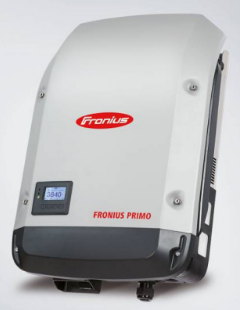
\includegraphics[width=0.5\textwidth]{figuras/inversor.PNG}
\caption{Inversor Fronius Primo 8.2-1 (8.200W)}
\end{figure}
Entrada:
\begin{itemize}
\item Voltagem máxima de entrada: 1000Vcc
\item Faixa de Voltagem do MPP: (270Vcc a 800Vcc)
\item Voltagem mínima de entrada: 80Vcc
\item Voltagem para inicialização: 80Vcc
\item Corrente máxima de entrada: 18A / 18A
\end{itemize}
Saída:
\begin{itemize}
\item Potência nominal de saída: 6000W
\item Voltagem de saída (faixa): 180Vca a 270Vca
\item Frequência de saída: 60Hz
\item Corrente máxima de saída: 35,7A
\end{itemize}
Outras características:
\begin{itemize}
\item Eficiência Máxima: 98,1\%
\item Consumo interno (noite): <1W
\item Temperatura de Operação: $-40\,^{\circ}\mathrm{C}$ a $+55\,^{\circ}\mathrm{C}$
\item Frequência de saída: 60Hz
\item Fabricante: Fronius
\end{itemize}
Especificações Mecânicas:
\begin{itemize}
\item Dimensões (L x A x P)mm: (645 x 431 x 204)
\item Peso: 21,5 kg
\end{itemize}

\subsection{Fiação elétrica}

\begin{figure}[h]
\centering
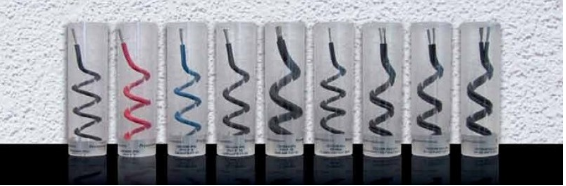
\includegraphics[width=0.5\textwidth]{figuras/cabo.PNG}
\caption{Cabo Solar Prysmian Afumex 4 mm$^2$ 1kV}
\end{figure}

\begin{itemize}
\item Temperatura máxima do condutor: $+120\,^{\circ}\mathrm{C}$
\item Resistência aos raios UV 720h
\item Performance contra fogo: Não propagante à chama, conforme EN 60332-1-2
\item Emissão de gases Halogênicos:  EN50525-1
\item Bitola: 4mm$^2$
\item Material: Cobre estanhado
\item Diâmetro externo: 5,9mm
\item Peso: 61kg/km
\item Corrente: 48 ~ 53 Variando com a temperatura
\item Cor: vermelho
\item Número de condutores: 1
\item Rcc máx a $20\,^{\circ}\mathrm{C}$: 5,09 ohm/km
\end{itemize}

\begin{figure}[h]
\centering
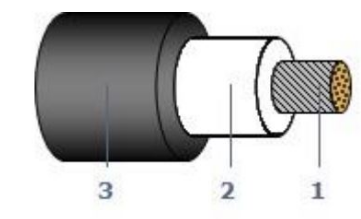
\includegraphics[width=0.5\textwidth]{figuras/composicaointerna.PNG}
\caption{Composição interna do cabo solar}
\end{figure}
Composição básica do cabo:
\begin{itemize}
\item Fio de Cobre estanhado, flexível
\\Enquadrado: Classe 5 - ABNT NBR-NM 280
\item Composto Termofixo HEPR $120\,^{\circ}\mathrm{C}$ - EN 50618 - 0,7mm
\item Composto Termofixo XLPE $120\,^{\circ}\mathrm{C}$
\\Enquadrado: EN 50618
\\Resistente aos Raios Ultravioletas (UV) - 0,8mm
\end{itemize}

\subsection{Suporte de angulação ajustável}

\begin{figure}[h]
\centering
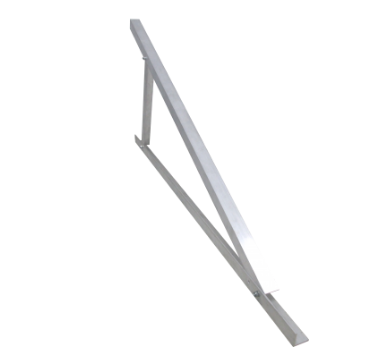
\includegraphics[width=0.5\textwidth]{figuras/angulacao.PNG}
\caption{Suporte de angulação ajustável de $15,^{\circ}$ e $20\,^{\circ}$}
\end{figure}

Confeccionado em alumínio, é utilizado em casos onde os módulos precisam ser montados em uma angulação maior que a do telhado. Ele é adaptável a qualquer tipo de telhado, pois pode ser usado em conjunto com os demais suportes para telhados, e também pode ser usado em terraços ou coberturas planas.

\par Na base inferior não há furação, pois é necessário saber a posição para furar o suporte no local certo do telhado. Na parte superior existem furações para fixar os perfis de alumínio, que serão os suportes dos módulos fotovoltaicos.

\subsection{Presilhas para módulos fotovoltaicos}

\begin{figure}[h]
\centering
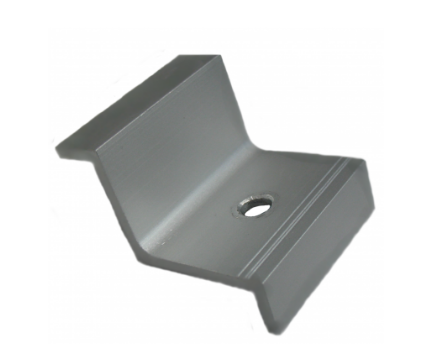
\includegraphics[width=0.5\textwidth]{figuras/presilha.PNG}
\caption{Presilha Lateral para Módulos Fotovoltaicos - Aba 40mm (Para Parafusos M8)}
\end{figure}

São utilizadas para fixar as módulos (placas) fotovoltaicas com aba de espessura de 40mm na estrutura. As presilhas laterais são montadas nas extremidades dos módulos fotovoltaicos, e são anodizadas com uma camada classe A23, segundo a norma NBR 12609.

\subsection{String Box (quadro elétrico fotovoltaico)}

\begin{figure}[h]
\centering
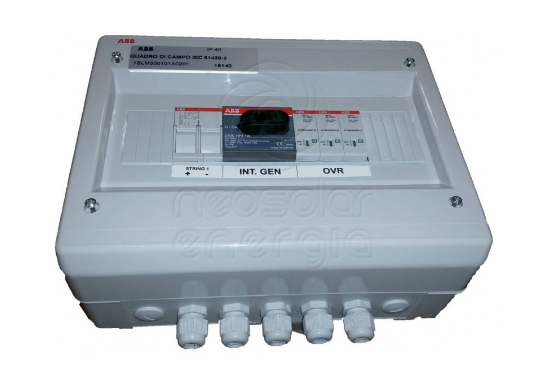
\includegraphics[width=0.5\textwidth]{figuras/stringbox.PNG}
\caption{Stringbox}
\end{figure}
Componentes

\begin{itemize}
\item par de porta-fusível com 1 par de fusíveis 10A
\item chave seccionadora corrente contínua
\item DPS corrente contínua para pólos positivos  e negativos
\item caixa elétrica IP40
\item prensa cabos, já instalados na parte interna da caixa
\end{itemize}

\section{Geração de energia}
O prédio do Restaurante Universitário disponibilizará de vinte painéis fotovoltaicos dispostos em duas strings (em série) e uma string em paralelo, será necessário para esse arranjo um inversor. A capacidade de geração de energia desse conjunto vai ser de 5,3 kWh.

\par No UED serão instaladas duzentas e cinquenta placas com capacidade de geração de 66,250 kWh. Com vinte e cinco strings, dez strings em paralelo e necessitando de dez inversores.

\par O UAC será o prédio com a maior geração de energia, uma vez que nele serão instaladas trezentas e cinquenta placas dispostas em trinta e cinco strings, dezoito strings em paralelo com dezoito inversores. A energia gerada pelos painéis será de 92,750 kWh.

\par Esse sistema se mostrou bastante eficiente, com uma capacidade geradora de energia de 164,3 kWh por mês. Combinado com o sistema de automação Smart Grid e a outra fonte de energia -- o biogás produzido a partir do biodigestor -- será possível reduzir os custos do consumo de energia demandando pela faculdade.

\begin{figure}[h]
\centering
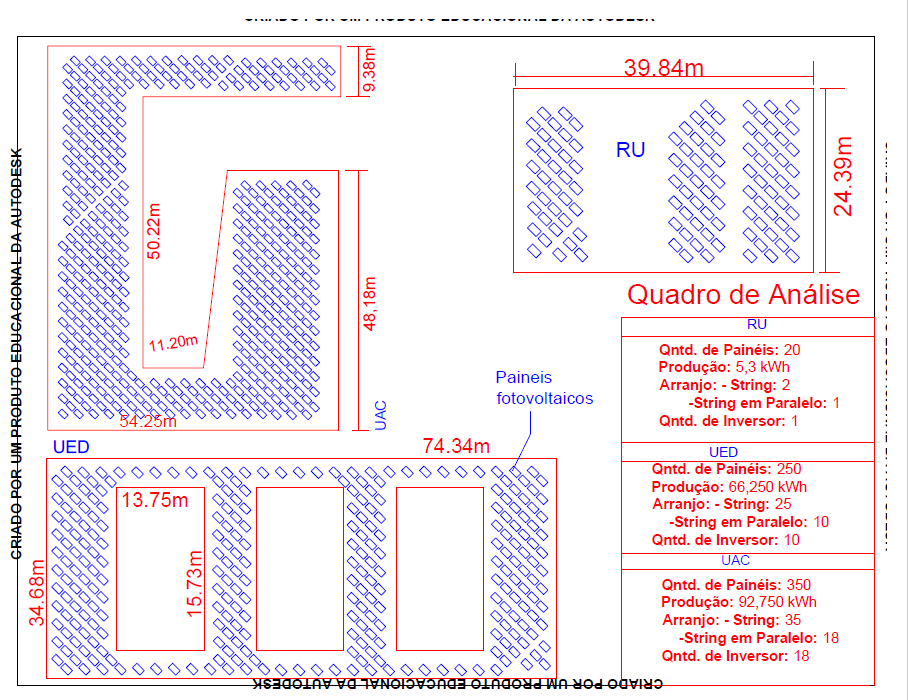
\includegraphics[width=0.9\textwidth]{figuras/disposicao.PNG}
\caption{Disposição dos paineis}
\end{figure}